% IEEE conference-style project report. Single file: upload to Overleaf (IEEEtran is built in)
% or compile with: pdflatex report.tex (twice).
% Every number comes from PROPOSAL.md; change them there first, then here.
\documentclass[conference]{IEEEtran}
\usepackage[utf8]{inputenc}
\usepackage[T1]{fontenc}
\usepackage{amsmath,amssymb}
\usepackage{booktabs}
\usepackage{graphicx}
\usepackage{cite}
\usepackage{url}
\usepackage{tikz}
\usetikzlibrary{positioning}

\newcommand{\ci}[2]{[#1,\,#2]}

\begin{document}

\title{Edition Confusion in Emerging-Entity Linking:\\
A Diagnosis and a Training-Free Reorder on TempEL}

\author{
\IEEEauthorblockN{Aaryan Degama}
\IEEEauthorblockA{\textit{B.Tech. IT-BI}\\
\textit{Indian Institute of Information}\\
\textit{Technology Allahabad}\\
Prayagraj, India\\
iib2024023@iiita.ac.in}
\and
\IEEEauthorblockN{Geethika Gorakala}
\IEEEauthorblockA{\textit{B.Tech. IT-BI}\\
\textit{Indian Institute of Information}\\
\textit{Technology Allahabad}\\
Prayagraj, India\\
iib2024024@iiita.ac.in}
\and
\IEEEauthorblockN{Archee Jaiswal}
\IEEEauthorblockA{\textit{B.Tech. IT-BI}\\
\textit{Indian Institute of Information}\\
\textit{Technology Allahabad}\\
Prayagraj, India\\
iib2024022@iiita.ac.in}
}

\maketitle

\begin{abstract}
Entity linkers lose accuracy as the knowledge base changes, and newly emerging entities lose the most:
the TempEL benchmark reports a drop of up to 17.9 accuracy@64 points for new entities against 3.1 for
continual ones. This report studies one cause of that drop and one problem in how it is evaluated.
First, on TempEL's full pool of 6,180,587 entities we reproduce the published accuracy@64
(0.7345 and 0.7673 against 0.734 and 0.767) and measure where new entities fail. For new entities that
are editions of a recurring event, a different edition of the same series holds rank~1 for 18.7\% of
mentions, while the correct page holds it for 12.8\%. We call this \emph{edition confusion}.
Second, we propose a training-free reorder that only permutes candidates inside a title family. In a
single pre-registered test pass it raises new-entity accuracy@1 from 0.174 to 0.210
(+3.6 points, 95\% CI \ci{+1.8}{+5.6}, $p = 0.0001$) and gains 2.5 points on the continual mentions it
can reorder. A prior that simply prefers the edition of the snapshot year matches it on new entities
but loses accuracy on continual ones.
Third, we re-run the public TIGER code and score new-entity mentions separately. The published
``new entity'' test set is 97\% continual mentions; R@1 on new-entity mentions alone is 0.34--0.35 where
the pooled figure is 0.19--0.20; and TIGER minus BLINK is below one point in our single-seed re-run.
We also report where the method does not win: on TIGER's pool of 10,373 entities a plain title matcher
gains more than our method.
\end{abstract}

\begin{IEEEkeywords}
entity linking, temporal drift, emerging entities, re-ranking, evaluation methodology, TempEL
\end{IEEEkeywords}

% ---------------------------------------------------------------------------------------------
\section{Introduction}

Entity linking (EL) maps a mention in text, such as ``Serie B'' in a football report, to the page of a
knowledge base that it refers to. Modern linkers first \emph{retrieve} a short candidate list from the
whole knowledge base with a dense bi-encoder \cite{blink} and then pick the top candidate.
Knowledge bases are not static. Wikipedia gains new pages every year, and a model trained on one
snapshot is later used on another. TempEL \cite{tempel} measures this and shows that \emph{new}
entities, the pages that did not exist when the model was trained, suffer far more than
\emph{continual} entities that exist in every snapshot.

TempEL's manual analysis also says what these new entities are: about 90\% are new members of an
existing family, either the next edition of a recurring event (about 68\%) or a page split off from an
older page (about 22\%) \cite{tempel}. This suggests a specific failure. The right page, for example
``2020--21 Serie B'', may already be in the candidate list but lose rank~1 to another edition of the
same series such as ``2018--19 Serie B''. TempEL's appendix guesses at this cause but does not measure
it, and the later graph-based linkers TIGER \cite{tiger} and CYCLE \cite{cycle} do not report where in
the ranking new entities fail.

This report makes three contributions, each tied to a published number.
\begin{itemize}
\item \textbf{C1, evaluation.} The first scores for TIGER and BLINK on new-entity mentions only.
We verified in TIGER's code and data that the published ``new entity'' test set contains 46,765
continual and 1,450 new mentions.
\item \textbf{C2, diagnosis.} A measured breakdown of why new entities fail on TempEL's full Wikipedia
pool, after reproducing TempEL's published accuracy.
\item \textbf{C3, method.} A training-free within-family reorder, judged by one pre-registered test
against four controls.
\end{itemize}

\textbf{Convention.} A number followed by a citation is quoted from that paper. Every other number was
measured in this work. Statements marked \emph{inferred} are our reading and were not measured. We make
no performance predictions.

\textbf{Code.} The code, the pre-registration and the full result tables are available at
\url{https://github.com/Aaryan-Degama/RM}.

% ---------------------------------------------------------------------------------------------
\section{Base Paper and Background}

\subsection{TempEL, the base paper}

TempEL \cite{tempel} is built from ten yearly snapshots of English Wikipedia, 2013 to 2022. Each
snapshot has its own entity pool (all pages of that year) and its own mentions (Table~\ref{tab:tempel}).
The model is a BLINK bi-encoder \cite{blink} on BERT-large \cite{bert}: one encoder turns the mention
and 128 tokens of context into a vector, another turns each entity description into a vector, and
candidates are ranked by dot product. The published metric is accuracy@64, the share of mentions whose
correct page is among the top 64 candidates retrieved from the whole snapshot.

\begin{table}[t]
\caption{TempEL data per snapshot \cite{tempel}}
\label{tab:tempel}
\centering
\begin{tabular}{lrrr}
\toprule
 & Train & Validation & Test \\
\midrule
Continual entities & 10,000 & 10,000 & 10,000 \\
Continual-entity mentions & 136,227 & 42,096 & 46,765 \\
New entities & 373 & 373 & 373 \\
New-entity mentions & 1,764 & 1,231 & 1,450 \\
\bottomrule
\end{tabular}
\end{table}

The findings of TempEL that motivate this work are the following, all reported in \cite{tempel}.
\begin{itemize}
\item Over time, continual entities lose up to 3.1 accuracy@64 points and new entities lose up to 17.9.
\item In a manual check of 100 new entities, about 68\% were recurring events and about 22\% were
extracts of existing pages.
\item In 2021, COVID-19 entities are 24\% of new entities and 30\% of their mentions, with about 14
extra points lost. These need new world knowledge, not disambiguation.
\item The overlap between the top-64 candidates of different mentions rises every year, so candidate
lists get more crowded with look-alike pages.
\end{itemize}

\subsection{Later work on the same benchmark}

\textbf{TIGER} \cite{tiger} and \textbf{CYCLE} \cite{cycle} train the bi-encoder with graph
information so that entity embeddings drift less over time. They evaluate on a reduced version of
TempEL and report recall@1 (R@1). For models trained on new-entity mentions and tested three years
later, the published R@1 is 0.142 for BLINK, 0.217 for TIGER and 0.222 for CYCLE \cite{tiger,cycle}.

\textbf{RAED} \cite{raed} generates descriptions for emerging entities with retrieval. For the 2019
model it reports emerging-entity accuracy@64 of 57.0, 47.4 and 53.5 on 2020, 2021 and 2022
\cite{raed}. Its retrieval index is a January 2023 dump, which is later than the test snapshots, and it
reports accuracy@64 only, so we make no numeric comparison with it.

% ---------------------------------------------------------------------------------------------
\section{Problems in the Existing Work}

We read TIGER's public code and released data \cite{tigercode,tigerdata} and found four issues that
shape this project. All four were checked directly in the code, the data or the supplementary tables.

\begin{enumerate}
\item \textbf{The ``new entity'' test set is pooled.} The ``new entities'' columns of
\cite{tiger,cycle} come from models \emph{trained} on 1,764 new-entity mentions but \emph{tested} on
46,765 continual plus 1,450 new mentions. So 97\% of the test mentions are continual, and the column
does not show how well new entities are linked.
\item \textbf{The candidate pool is small.} It holds 10,373 entities, against 6,180,587 in TempEL's own
2021 evaluation. A small pool that consists only of test answers has few distractors.
\item \textbf{The three-year gap is a single train/test pair,} 2019 to 2022.
\item \textbf{CYCLE cannot be re-run.} Its public repository lacks the model source folder (checked on
2026-11-06). CYCLE is therefore quoted, not re-run.
\end{enumerate}

Beyond these, no prior work reports \emph{where in the ranking} new entities fail: whether the correct
page was not retrieved at all, or was retrieved and then lost to a sibling page.

% ---------------------------------------------------------------------------------------------
\section{Problem Statement and Focus}

\textbf{Task.} The input is a mention with its context, observed in snapshot $t$, and the top-$K$
candidates from the knowledge base of snapshot $t$ under TempEL's frozen 2019 bi-encoder
($K = 64$, and $K = 256$ in Section~\ref{sec:d256}). The output is a re-ordering of that list.
Nothing dated after $t$ is used and nothing is trained.

We separate three populations.
\begin{itemize}
\item \textbf{P1, continual entities.} They must not get worse. They appear in every table.
\item \textbf{P2, new members of a family} (recurring events, page extracts). The main target.
\item \textbf{P3, genuinely novel entities} (COVID-19). Reported as a separate slice; our method does
not address them.
\end{itemize}

\textbf{Research questions.}
\begin{itemize}
\item \textbf{RQ1 (diagnosis).} What share of new-entity errors are retrieval misses, edition
confusions, or other ranking errors?
\item \textbf{RQ2 (method).} Does a training-free within-family reorder raise new-entity accuracy@1
over the frozen model, and over simple priors that exploit how the benchmark is built?
\item \textbf{RQ3 (safety).} Does it leave continual entities at least as accurate?
\item \textbf{RQ4 (evaluation).} What do BLINK and TIGER score on new-entity mentions alone?
\end{itemize}

We focus on the ranking step, not on retrieval or on new training, for two reasons. The diagnosis
(Section~\ref{sec:diag}) shows a measurable share of errors that a reorder can reach, and a reorder
needs no GPU, which fits a project run on one laptop.

% ---------------------------------------------------------------------------------------------
\section{Methodology}

\subsection{Reproduction pipeline}

Fig.~\ref{fig:pipe} shows the pipeline. We use TempEL's released 2019 model and its released entity
encodings for the 2021 snapshot (6,180,587 vectors of 1,024 dimensions, a 25.3~GB file). We encode all
48,215 test mentions of 2021 with the frozen mention encoder, using TempEL's own tokenization, and run
an exact (not approximate) top-256 search over the memory-mapped encoding table. Steps 1 and 2 ran
once and are cached. Steps 3 and 4 take minutes on a laptop CPU.

\begin{figure}[t]
\centering
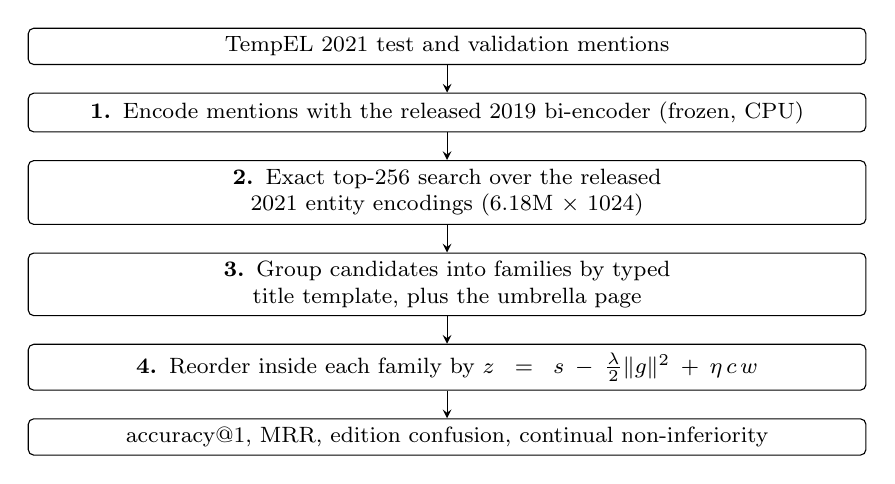
\begin{tikzpicture}[node distance=3.5mm,
  box/.style={draw, rounded corners=2pt, align=center, font=\footnotesize, text width=0.86\columnwidth, inner sep=3pt},
  >=stealth]
\node[box] (a) {TempEL 2021 test and validation mentions};
\node[box, below=of a] (b) {\textbf{1.} Encode mentions with the released 2019 bi-encoder (frozen, CPU)};
\node[box, below=of b] (c) {\textbf{2.} Exact top-256 search over the released 2021 entity encodings (6.18M $\times$ 1024)};
\node[box, below=of c] (d) {\textbf{3.} Group candidates into families by typed title template, plus the umbrella page};
\node[box, below=of d] (e) {\textbf{4.} Reorder inside each family by $z = s - \tfrac{\lambda}{2}\lVert g\rVert^2 + \eta\,c\,w$};
\node[box, below=of e] (f) {accuracy@1, MRR, edition confusion, continual non-inferiority};
\draw[->] (a) -- (b); \draw[->] (b) -- (c); \draw[->] (c) -- (d); \draw[->] (d) -- (e); \draw[->] (e) -- (f);
\end{tikzpicture}
\caption{The pipeline. Nothing is trained; the retrieved list is only re-ordered.}
\label{fig:pipe}
\end{figure}

\subsection{Families from typed title slots}

A title word is a \emph{slot} if it is a year, a season (``2019--20''), an ordinal (``23rd''), a plain
number, a Roman numeral of two or more letters, or a number word. Words that mix letters and digits
(``COVID-19'', ``F-16'') are never slots. Replacing the slots by \# gives the title's \emph{template}:
``2022 FIFA World Cup'' becomes ``\# FIFA World Cup''.

Candidates in the list that share a template and slot types form a \emph{family}. The \emph{umbrella
page}, the template without its slot (``FIFA World Cup''), joins the family. Families that share a
member are merged. A family needs at least two members, one of them with a slot.

\subsection{Slot evidence}

For a candidate $e$ with a slot, the evidence $w(e) \in [0,1]$ says whether its slot value appears in
the 128 tokens the encoder saw. It is 1 if the exact value occurs inside the mention span and
$\tfrac12$ if it occurs elsewhere in the window. A bare year that is only one end of a season counts
half. Non-year slots count only inside the mention span. The umbrella page has $w = 0$.

\subsection{Score and ordering}

Inside a family, candidates are sorted by
\begin{equation}
z(e) = s(e) - \frac{\lambda}{2}\,\lVert g_e \rVert^2 + \eta\, c\, w(e),
\label{eq:z}
\end{equation}
where $s(e)$ is the frozen dot-product score and $g_e$ the entity vector. With $\lambda = 1$ the first
two terms rank a family by Euclidean distance instead of dot product, which removes the advantage of
entities with long vectors. The constant $c$ is the median gap between the first and second score on
validation (2.10 for TempEL); it needs no labels and only sets the unit of $\eta$.

Each family refills \emph{exactly the list positions it already holds}, sorted by $z$. Candidates
outside a family never move. This gives four guarantees, which the code asserts on every run:
\begin{enumerate}
\item non-family candidates keep their positions;
\item accuracy@$K$ at the list depth cannot change;
\item any change in accuracy@1 is a swap between siblings;
\item $\lambda = \eta = 0$ reproduces the frozen list exactly.
\end{enumerate}

The two knobs were tuned on validation only, over $\eta \in \{0, 0.5, 1, 2, 4, \infty\}$ and
$\lambda \in \{0, 0.25, 0.5, 1\}$. Every fold selected $\eta = \infty$ and $\lambda = 0.5$: inside a
family, candidates whose slot is supported by the context come first, and the corrected score breaks
ties.

Table~\ref{tab:example} shows one test mention. The frozen model puts the umbrella page first and the
correct edition at rank 17. The context contains ``2020--21'', so the reorder moves that edition into
the first family position. Candidates outside the family keep their ranks.

\begin{table}[t]
\caption{One new-entity test mention: ``Serie B'' in a text about the 2020--21 season of a club.
Correct page: ``2020--21 Serie B'' (rank 17 $\rightarrow$ 1). F marks family members.}
\label{tab:example}
\centering
\footnotesize
\begin{tabular}{cll}
\toprule
Rank & Frozen TempEL model & After the reorder \\
\midrule
1 & Serie B (F) & \textbf{2020--21 Serie B} (F) \\
2 & Serie B (disambiguation) & Serie B (disambiguation) \\
3 & 2018--19 Serie B (F) & 2019--20 Serie B (F) \\
4 & Lega B & Lega B \\
5 & List of Serie B champions \ldots & List of Serie B champions \ldots \\
\bottomrule
\end{tabular}
\end{table}

\subsection{Controls}

A gain could come from the benchmark's construction and not from the mention's context. Each control
below tests one such explanation. All use the same within-family ordering unless stated, and each was
tuned on validation by the same rule.
\begin{itemize}
\item \textbf{Recency prior:} prefer the largest slot value in the family. Is the gain just ``pick the
newest edition''?
\item \textbf{Snapshot-year prior:} prefer editions dated 2020. Is the gain just the benchmark's year?
\item \textbf{Placebo:} slot evidence taken from the context of a different entity's mention. Does the
mention's own context matter?
\item \textbf{Title-matcher:} slot evidence applied to the whole list, with no families. Do families
matter?
\item \textbf{$\lambda$-only and $\eta$-only:} which term carries the effect?
\end{itemize}

\subsection{Evaluation protocol}

The rules were committed to git (commit \texttt{12fd858}, 2026-11-07) before the test split was scored.
\begin{itemize}
\item \textbf{Data:} TempEL 2021 test, 2019 model, full pool, top-64; all 1,450 new and 46,765
continual mentions.
\item \textbf{Primary test:} change in new-entity accuracy@1, method minus frozen; entity-level
sign-flip permutation test with 10,000 permutations, two-sided, $\alpha = 0.05$.
\item \textbf{Non-inferiority:} on continual mentions whose rank-1 candidate lies in a family
(``changeable''), the lower end of the 95\% interval of the change must be at least $-1.0$ point.
\item \textbf{Cross-fitting:} validation and test share entities, so knobs are chosen in five folds
grouped by title template; a mention is scored with knobs chosen on the other folds.
\item \textbf{Secondary tests:} method against each control, Holm-corrected \cite{holm} over 12 tests.
\item \textbf{One test pass.} Anything later is labelled exploratory.
\end{itemize}

There are only 373 new entities, so all intervals are 95\% bootstrap intervals that resample
\emph{entities}, not mentions, and all tests are paired. Everything used at test time is dated on or
before 2021-01-01: the pool, the titles and the released encodings. The backbone is BERT-large,
pretrained on 2018 Wikipedia. No large language model is used.

\subsection{Re-scoring under TIGER's protocol}

For C1 we ran TIGER's own code at a fixed commit \cite{tigercode} with its released data
\cite{tigerdata} and its own configuration files for BLINK and TIGER (seed 52313, one epoch). We
trained on \{new, continual\} mentions for each of the years 2019--2022, 16 models in total, and
tested each forward in time on TIGER's pool of 10,373 entities. A three-line patch saves the top-64
list of every test mention, so pooled, new-only and continual-only R@1 come from the same pass. The
run used a free Kaggle T4 GPU. We ran one seed.

% ---------------------------------------------------------------------------------------------
\section{Results}

\subsection{Reproduction of TempEL}

Table~\ref{tab:repro} shows that our pipeline reproduces the published accuracy@64 to three decimals.
TempEL reports accuracy@64 only. From the same run, the frozen model's accuracy@1 is 0.1738 for new
and 0.2117 for continual entities.

\begin{table}[t]
\caption{Reproduction: 2019 model, 2021 test, full pool, accuracy@64}
\label{tab:repro}
\centering
\begin{tabular}{lcc}
\toprule
 & Ours & TempEL \cite{tempel} \\
\midrule
New entities (1,450 mentions) & 0.7345 & 0.734 \\
Continual entities (46,765 mentions) & 0.7673 & 0.767 \\
\bottomrule
\end{tabular}
\end{table}

\subsection{C2: why new entities fail}
\label{sec:diag}

Table~\ref{tab:diag} places every test mention in exactly one bucket. ``Edition confusion'' means that
the rank-1 candidate is in the correct page's family: another edition or the umbrella page.

\begin{table*}[t]
\caption{Error diagnosis of the frozen model on the 2021 test set (full pool, top-64). Each mention falls in exactly one of the five middle columns.}
\label{tab:diag}
\centering
\begin{tabular}{lrcccccc}
\toprule
Slice & $n$ & Correct & Edition & Other error, & Miss, a sibling & Miss, & Ceiling of a perfect \\
 & & at 1 & confusion at 1 & gold in top-64 & in top-64 & no sibling & family reorder (acc@1) \\
\midrule
New: recurrent & 561 & 12.8\% & \textbf{18.7\%} & 48.0\% & 10.5\% & 10.0\% & 0.316 \\
New: COVID & 440 & 17.0\% & 0.0\% & 45.2\% & 0.0\% & \textbf{37.7\%} & 0.171 \\
New: other & 449 & 23.4\% & 3.6\% & 49.9\% & 2.2\% & 20.9\% & 0.270 \\
New: all & 1,450 & 17.4\% & 8.3\% & 47.7\% & 4.8\% & 21.8\% & 0.257 \\
Continual & 46,765 & 21.2\% & 2.8\% & 52.8\% & 1.6\% & 21.7\% & 0.240 \\
\bottomrule
\end{tabular}
\end{table*}

\begin{itemize}
\item \textbf{Recurrent new entities:} a wrong edition wins rank~1 more often than the right page
does (18.7\% against 12.8\%). Validation shows the same pattern (22.9\% against 9.8\%).
\item \textbf{COVID new entities:} no edition confusion at all. The main failure is that the correct
page is not retrieved (37.7\%). A reorder cannot help this population.
\item \textbf{Headroom:} a perfect within-family reorder would lift new-entity accuracy@1 from 0.174
to 0.257. About half of all errors are neither misses nor edition confusions and are outside the reach
of this method.
\end{itemize}

\subsection{C3: the pre-registered test}

Table~\ref{tab:main} gives the single test pass. Accuracy@64 is 0.7345 in every row, as guaranteed.

\begin{table*}[t]
\caption{The pre-registered test: 2019 model, 2021 test, full pool, depth 64. $\Delta$ are points of accuracy@1 against the frozen model with 95\% entity-bootstrap intervals. ``Changeable continual'' are the 10,111 continual mentions whose rank-1 candidate lies in a family.}
\label{tab:main}
\centering
\footnotesize
\begin{tabular}{lccccccc}
\toprule
Row & New & $\Delta$ new & New & New edition & Fixed / created & $\Delta$ changeable & Continual \\
 & acc@1 & [95\% CI] & MRR & confusion at 1 & (new) & continual [95\% CI] & acc@1 \\
\midrule
Frozen TempEL & 0.1738 & -- & 0.274 & 8.3\% & -- & -- & 0.2117 \\
Recency prior & 0.1807 & $+0.7$ \ci{+0.1}{+1.3} & 0.287 & 7.7\% & 13 / 3 & $-0.2$ \ci{-0.4}{-0.1} & 0.2113 \\
Snapshot-year prior & 0.2062 & $+3.2$ \ci{+1.8}{+4.9} & 0.319 & 5.1\% & 47 / 0 & $-0.3$ \ci{-0.4}{-0.1} & 0.2111 \\
Placebo & 0.1710 & $-0.3$ \ci{-0.7}{+0.1} & 0.274 & 8.6\% & 2 / 6 & $-0.3$ \ci{-0.6}{+0.1} & 0.2111 \\
Title-matcher (whole list) & 0.1834 & $+1.0$ \ci{+0.1}{+2.0} & 0.287 & 7.7\% & 23 / 9 & $+2.4$ \ci{+1.9}{+3.0} & 0.2192 \\
$\lambda$-only & 0.1724 & $-0.1$ \ci{-0.6}{+0.2} & 0.275 & 8.5\% & 3 / 5 & $+0.0$ \ci{-0.3}{+0.3} & 0.2118 \\
$\eta$-only & 0.2034 & $+3.0$ \ci{+1.5}{+4.6} & 0.311 & 5.4\% & 43 / 0 & $+2.7$ \ci{+2.1}{+3.4} & 0.2176 \\
\textbf{Ours} & \textbf{0.2097} & $\mathbf{+3.6}$ \ci{+1.8}{+5.6} & 0.317 & \textbf{4.8\%} & 52 / 0 & $+2.5$ \ci{+1.9}{+3.2} & 0.2172 \\
\midrule
Ceiling (perfect reorder) & 0.2572 & $+8.3$ & & & & & \\
\bottomrule
\end{tabular}
\end{table*}

\textbf{Against the pre-registered rules.}
The primary test passed: $+3.6$ points, $p = 0.0001$. The non-inferiority test passed: the lower end
of the interval on changeable continual mentions is $+1.9$, against a limit of $-1.0$. On new
entities the method fixed 52 mentions and created no error. On continual entities it does create
errors: 424 fixed against 168 created, so the net is positive but ``creates no errors'' holds for new
entities only.

\textbf{Against the controls} (Table~\ref{tab:sec}).
The method beats the recency prior, the placebo and the title-matcher on all new mentions after
correction for multiple tests. It does \emph{not} beat the snapshot-year prior ($+0.3$, not
significant).

\begin{table}[t]
\caption{Secondary tests: our method minus each control, points of new-entity accuracy@1, all 1,450 new mentions. $p$ values are Holm-corrected over 12 tests.}
\label{tab:sec}
\centering
\begin{tabular}{lcc}
\toprule
Against & Difference [95\% CI] & $p$ \\
\midrule
Recency prior & $+2.9$ \ci{+1.4}{+4.5} & 0.001 \\
Snapshot-year prior & $+0.3$ \ci{-1.4}{+2.2} & n.s. \\
Placebo & $+3.9$ \ci{+2.1}{+5.9} & 0.001 \\
Title-matcher & $+2.6$ \ci{+1.0}{+4.4} & 0.02 \\
\bottomrule
\end{tabular}
\end{table}

\textbf{Reading the result.}
The mention's own context matters, because the placebo gains nothing. Families matter, because the
title-matcher gains about a third as much on new entities. The effect is carried by the slot
evidence: the norm term adds 0.6 points on top of $\eta$-only, which we did not test for significance.

The tie with the snapshot-year prior has a clear cause. TempEL's new entities are, by construction,
pages created in the last year, and we measured that 81\% of the dated new correct titles are 2020
editions. A prior that knows the snapshot year captures most of the available gain. The two rules
differ on continual entities: the prior loses 0.3 points there and our method gains 2.5 (the
difference, $+2.8$ \ci{+2.1}{+3.5}, is descriptive and was not pre-registered). The prior uses no
context, so it wrongly prefers 2020 editions for mentions of older events; our method reads the year
from the context. The claim we can defend is therefore that this is \emph{the only tested rule that
helps both populations}, not that it beats every baseline.

\subsection{Depth 256: the published metric}
\label{sec:d256}

Re-ordering the top 64 cannot change accuracy@64. Re-ordering the top 256 can, and accuracy@64 is the
metric TempEL publishes. The depth-64 knobs were applied unchanged to the top-256 lists in one pass
(Table~\ref{tab:d256}). Our method lifts new-entity accuracy@64 from 0.7345 to 0.751 with continual
entities unchanged. The snapshot-year prior is higher still on new entities (0.764), again at a small
but significant cost on continual entities.

\begin{table}[t]
\caption{Accuracy@64 after re-ordering the top 256 (2021 test). $\Delta$ in points against the frozen model, 95\% CI.}
\label{tab:d256}
\centering
\footnotesize
\begin{tabular}{lcccc}
\toprule
 & New & $\Delta$ new & Cont. & $\Delta$ continual \\
\midrule
TempEL \cite{tempel} & 0.734 & & 0.767 & \\
Frozen (ours) & 0.7345 & -- & 0.7673 & -- \\
Recency prior & 0.7441 & $+1.0$ \ci{+0.2}{+1.8} & 0.7669 & $-0.04$ \\
Snapshot-year & 0.7641 & $+3.0$ \ci{+1.4}{+5.0} & 0.7667 & $-0.06$ \\
Title-matcher & 0.7386 & $+0.4$ \ci{-0.3}{+1.2} & 0.7695 & $+0.21$ \\
\textbf{Ours} & \textbf{0.7510} & $+1.7$ \ci{+0.6}{+3.0} & 0.7677 & $+0.04$ \\
Ceiling & 0.7717 & $+3.7$ & 0.7787 & $+1.1$ \\
\bottomrule
\end{tabular}
\end{table}

\subsection{C1: TIGER and BLINK on new-entity mentions only}

Table~\ref{tab:c1} gives R@1 for models trained on new-entity mentions, averaged over train/test
pairs with the same forward gap, which is the convention of \cite{tiger,cycle}. The test set is the
same 48,215 mentions in every row; only the mentions that are counted differ.

\begin{table}[t]
\caption{R@1 under TIGER's protocol (pool of 10,373 entities), models trained on new-entity mentions. Gap = test year minus train year. Published rows are from \cite{tiger,cycle}; re-run rows are ours (one seed).}
\label{tab:c1}
\centering
\footnotesize
\begin{tabular}{llcccc}
\toprule
Model & Scored on & Gap 0 & Gap 1 & Gap 2 & Gap 3 \\
\midrule
BLINK, published & pooled & .132 & .132 & .132 & .142 \\
BLINK, re-run & pooled & .204 & .203 & .193 & .193 \\
 & \textbf{new only} & \textbf{.323} & \textbf{.296} & \textbf{.297} & \textbf{.343} \\
 & continual only & .201 & .200 & .190 & .189 \\
\midrule
TIGER, published & pooled & .186 & .195 & .188 & .217 \\
TIGER, re-run & pooled & .204 & .202 & .196 & .199 \\
 & \textbf{new only} & \textbf{.333} & \textbf{.311} & \textbf{.329} & \textbf{.349} \\
 & continual only & .200 & .199 & .192 & .195 \\
\midrule
CYCLE, published & pooled & .184 & .191 & .192 & .222 \\
\bottomrule
\end{tabular}
\end{table}

\begin{itemize}
\item \textbf{The pooled score is the continual score.} In Table~\ref{tab:c1} the two differ by at
most 0.4 points. The published ``new entity'' column therefore describes how a model trained on
new-entity mentions does on continual mentions.
\item \textbf{On new-entity mentions alone, R@1 is 10 to 15 points higher} than the pooled figure
(0.30--0.35 against 0.19--0.20).
\item \textbf{The published gap between BLINK and TIGER did not reproduce in our re-run.} Our BLINK
re-run is 5 to 7 points above the published BLINK row, and our TIGER re-run is within 2 points of the
published TIGER row.
\end{itemize}

Table~\ref{tab:tb} compares the two models on the same mentions. In our re-run TIGER's gain is real
but under one point, and it sits on continual mentions. On new-entity mentions the difference cannot
be told from zero with 1,450 mentions. This does \emph{not} show that the published results are wrong:
we ran one seed of a re-released codebase on different hardware, and the larger mismatch is in the
BLINK baseline row.

\begin{table}[t]
\caption{TIGER minus BLINK in our re-run, points of R@1 on the same mentions (2019 models, 95\% entity-bootstrap CI).}
\label{tab:tb}
\centering
\footnotesize
\begin{tabular}{cccc}
\toprule
Test year & Pooled & New only & Continual only \\
\midrule
2019 & $+0.7$ \ci{+0.3}{+1.1} & $+0.7$ \ci{-2.6}{+4.0} & $+0.7$ \ci{+0.3}{+1.1} \\
2020 & $+0.7$ \ci{+0.3}{+1.1} & $-0.7$ \ci{-4.3}{+2.8} & $+0.8$ \ci{+0.4}{+1.2} \\
2021 & $+0.5$ \ci{+0.2}{+0.9} & $-1.9$ \ci{-4.9}{+0.9} & $+0.6$ \ci{+0.2}{+1.0} \\
2022 & $+0.6$ \ci{+0.2}{+1.0} & $+0.5$ \ci{-2.6}{+3.8} & $+0.6$ \ci{+0.2}{+1.0} \\
\bottomrule
\end{tabular}
\end{table}

\subsection{The method on TIGER's and BLINK's lists}

We applied the method to the top-64 lists of the 2019 new-trained models with the knobs chosen on
TempEL unchanged. Only $c$ was re-estimated, without labels, from each model's own validation lists
(0.774 for BLINK and 0.839 for TIGER). The script ran once (Table~\ref{tab:tigerb}).

\begin{table*}[t]
\caption{The reorder applied to BLINK's and TIGER's lists under TIGER's protocol, knobs unchanged from TempEL. Gains are points of new-entity R@1 over each model's own list, with 95\% CIs. ``Oracle'' is a perfect within-family reorder.}
\label{tab:tigerb}
\centering
\footnotesize
\begin{tabular}{lccccccc}
\toprule
Model, test year & New R@1 & Oracle & Ours & Snapshot-year & Title-matcher & \multicolumn{2}{c}{Continual R@1} \\
 & (frozen) & & & prior & (whole list) & frozen $\rightarrow$ ours & title-matcher \\
\midrule
BLINK, 2021 & .309 & .321 & $+0.4$ \ci{-0.2}{+1.1} & $+0.3$ \ci{-0.6}{+1.2} & $+5.2$ \ci{+3.4}{+7.5} & .192 $\rightarrow$ .212 & .240 \\
TIGER, 2021 & .290 & .307 & $+1.0$ \ci{+0.2}{+2.0} & $+0.8$ \ci{+0.1}{+1.5} & $+6.9$ \ci{+4.7}{+9.3} & .198 $\rightarrow$ .219 & .247 \\
BLINK, 2022 & .343 & .381 & $+2.1$ \ci{+0.9}{+3.5} & $+2.0$ \ci{+0.9}{+3.3} & $+9.8$ \ci{+7.4}{+12.3} & .189 $\rightarrow$ .209 & .235 \\
TIGER, 2022 & .349 & .383 & $+2.2$ \ci{+1.1}{+3.7} & $+1.3$ \ci{+0.4}{+2.4} & $+12.0$ \ci{+9.2}{+15.0} & .195 $\rightarrow$ .215 & .244 \\
\bottomrule
\end{tabular}
\end{table*}

\begin{itemize}
\item \textbf{The method transfers.} Over the four test years 2019--2022 and both models, new-entity
R@1 rises in all eight cells ($+0.4$ to $+2.2$) and seven of the eight intervals exclude zero.
Continual R@1 rises by 2.0 to 2.2 points in every cell.
\item \textbf{The room on new entities is small.} The correct page sits in an in-list family for only
13--22\% of new mentions, and a perfect within-family reorder would add 1.2 to 3.8 points.
\item \textbf{The title-matcher control beats the method on this pool,} by a wide margin ($+5$ to
$+12$ points on new entities). On TempEL's full pool the order was the reverse ($+1.0$ against
$+3.6$). \emph{Inferred, not tested:} in a pool of 10,373 pages that are all test answers, a page
whose year appears in the context is rarely a distractor; among 6.18 million pages it often is, and
the family restriction is what protects the ranking.
\item \textbf{A caution about the small pool.} A training-free title match adds 5 to 12 points of
new-entity R@1 here, several times the TIGER-minus-BLINK difference in our re-run. Scores on this
pool are very sensitive to surface title cues.
\end{itemize}

% ---------------------------------------------------------------------------------------------
\section{Comparison with Benchmarks}

Table~\ref{tab:comp} places each of our numbers next to the published number it can be compared with,
and says what kind of comparison it is. We use two benchmarks: TempEL's own evaluation (full pool,
accuracy@64) as the main one, and the TIGER/CYCLE protocol (small pool, R@1) as the second.

\begin{table*}[t]
\caption{Our numbers against the published benchmarks}
\label{tab:comp}
\centering
\footnotesize
\begin{tabular}{p{5.2cm}p{3.3cm}p{3.6cm}p{4.4cm}}
\toprule
Quantity & Published & Ours & Kind of comparison \\
\midrule
TempEL accuracy@64, new / continual (2019 model, 2021 test, full pool)
 & 0.734 / 0.767 \cite{tempel}
 & 0.7345 / 0.7673 (frozen)
 & Reproduction: same model, pool and data \\
Same metric after our reorder of the top 256
 & 0.734 / 0.767 \cite{tempel}
 & 0.751 / 0.768
 & Same metric as published; paired with our frozen run \\
Accuracy@1, new / continual (not published by TempEL)
 & --
 & 0.174 / 0.212 frozen; 0.210 / 0.217 ours
 & Paired, same lists \\
BLINK, pooled R@1, gap 3 (TIGER protocol)
 & 0.142 \cite{tiger}
 & 0.193 (re-run)
 & Reproduction check: same code, data and protocol; one seed \\
TIGER, pooled R@1, gap 3
 & 0.217 \cite{tiger}
 & 0.199 (re-run)
 & Reproduction check; one seed \\
CYCLE, pooled R@1, gap 3
 & 0.222 \cite{cycle}
 & not run
 & Public code cannot run \\
BLINK / TIGER, new-only R@1, gap 3
 & --
 & 0.343 / 0.349
 & New numbers; no published counterpart \\
Our reorder on TIGER's list, new R@1, 2022
 & --
 & 0.349 $\rightarrow$ 0.371
 & Paired with our re-run; knobs unchanged \\
RAED \cite{raed}
 & 57.0 / 47.4 / 53.5 (acc@64)
 & --
 & Not compared: different index and metric \\
\bottomrule
\end{tabular}
\end{table*}

Three points summarize the comparison.
\begin{itemize}
\item \textbf{Against TempEL:} our frozen run matches the published accuracy@64. On that same metric
the reorder at depth 256 gives 0.751 for new entities where TempEL publishes 0.734, with continual
entities unchanged.
\item \textbf{Against TIGER and CYCLE:} the reorder is not a competing model. It is applied on top of
a model's list, and on TIGER's own list it adds $+1.0$ to $+2.2$ points of new-entity R@1. We do not
claim to beat TIGER or CYCLE.
\item \textbf{About the benchmark itself:} scoring new-entity mentions separately changes the picture
of the TIGER/CYCLE protocol more than either model does.
\end{itemize}

% ---------------------------------------------------------------------------------------------
\section{Limitations}

\begin{itemize}
\item \textbf{The snapshot-year prior ties the method} on new-entity accuracy@1 and beats it on
accuracy@64. Part of what looks like edition confusion on TempEL is a recency artifact of how its new
entities are sampled.
\item \textbf{COVID and other novel entities are not helped.} They have no editions, and 37.7\% of
their mentions miss retrieval entirely.
\item \textbf{One cell on the full pool.} The pre-registered results are for the 2019 model on the
2021 snapshot. Other years were tested only on TIGER's small pool.
\item \textbf{On TIGER's pool a plain title matcher beats the method.} The method's advantage over
that control is specific to the large pool.
\item \textbf{The TIGER/BLINK re-run is one seed} of a re-released codebase. It does not establish
that the published numbers are wrong.
\item \textbf{Title templates only.} Page extracts whose titles share no template form no family and
are not touched.
\item \textbf{The ceiling is low.} Even a perfect within-family reorder reaches 0.257 accuracy@1.
\item \textbf{The hand audit is not finished.} A blind manual check of 100 sampled errors against the
automatic buckets of Table~\ref{tab:diag} is in progress. No number in this report depends on it.
\end{itemize}

We do not claim state of the art, and we make no numeric comparison with RAED.

% ---------------------------------------------------------------------------------------------
\section{Compute}

All TempEL-side work ran on one laptop (Ryzen 7 7730U, 15~GB RAM, no GPU). Encoding the 48,215 test
mentions took about 3~h~10~min, and the exact top-256 search over the 6.18M $\times$ 1024 table took
about 55~min. Family features, tuning and the test take minutes. Nothing was trained on the TempEL
side. The TIGER grid of 16 small models took about 2.6~h per run on a free Kaggle T4 GPU, and applying
the reorder to those lists took about 10~min on the laptop.

% ---------------------------------------------------------------------------------------------
\section{Conclusion and Future Work}

We reproduced TempEL on its full pool, measured that edition confusion is a real and specific failure
of recurring-event new entities (18.7\% of their mentions, more than the 12.8\% that are linked
correctly), and showed that a training-free within-family reorder recovers part of it: $+3.6$ points
of new-entity accuracy@1 in a pre-registered test, with a gain and not a loss on continual entities.
We also showed that the ``new entity'' column of the TIGER/CYCLE protocol is, in practice, a
continual-entity score, and gave the first new-only scores for BLINK and TIGER under that protocol.

The results come with two findings against our own method, which we report in full: a prior that
knows the snapshot year ties it on new entities, and on a small pool a plain title matcher beats it.

Future work: (1) other train/test years on the full pool; (2) a retrieval-side fix for misses that
have a sibling in the list (10.5\% of recurrent new mentions); (3) routing novel entities such as
COVID-19 to a knowledge-adding method with a temporally sound index; (4) a trained cross-encoder as an
upper-bound re-ranker, with and without the family reorder; (5) fine-tuning with sibling pages as hard
negatives.

\begin{thebibliography}{00}
\bibitem{tempel} K. Zaporojets, L.-A. Kaffee, J. Deleu, T. Demeester, C. Develder, and I. Augenstein,
``TempEL: Linking dynamically evolving and newly emerging entities,'' in \emph{Advances in Neural
Information Processing Systems (NeurIPS), Datasets and Benchmarks Track}, 2022.
\bibitem{tiger} P. Zhang, C. Cao, and P. Groth, ``TIGER: Temporally improved graph entity linker,'' in
\emph{Proc. European Conf. on Artificial Intelligence (ECAI)}, 2024.
\bibitem{cycle} P. Zhang, C. Cao, K. Zaporojets, and P. Groth, ``CYCLE: Cross-year contrastive learning
in entity-linking,'' in \emph{Proc. ACM Int. Conf. on Information and Knowledge Management (CIKM)},
2024, doi: 10.1145/3627673.3679702.
\bibitem{blink} L. Wu, F. Petroni, M. Josifoski, S. Riedel, and L. Zettlemoyer, ``Scalable zero-shot
entity linking with dense entity retrieval,'' in \emph{Proc. Conf. on Empirical Methods in Natural
Language Processing (EMNLP)}, 2020.
\bibitem{raed} K. Ghonim, P.-L. Huguet Cabot, R. Orlando, and R. Navigli, ``RAED: Retrieval-augmented
entity description generation for emerging entity linking and disambiguation,'' in \emph{Proc. Conf. on
Empirical Methods in Natural Language Processing (EMNLP)}, 2025.
\bibitem{bert} J. Devlin, M.-W. Chang, K. Lee, and K. Toutanova, ``BERT: Pre-training of deep
bidirectional transformers for language understanding,'' in \emph{Proc. NAACL-HLT}, 2019.
\bibitem{holm} S. Holm, ``A simple sequentially rejective multiple test procedure,''
\emph{Scandinavian Journal of Statistics}, vol. 6, no. 2, pp. 65--70, 1979.
\bibitem{tigercode} P. Zhang, ``TIGER: Temporally improved graph entity linker,'' source code,
commit 649bb19. [Online]. Available:
\url{https://github.com/pengyu-zhang/TIGER-Temporally-Improved-Graph-Entity-Linker}
\bibitem{tigerdata} P. Zhang, C. Cao, and P. Groth, ``TIGER data release,'' Zenodo, record 10977757.
[Online]. Available: \url{https://zenodo.org/records/10977757}
\end{thebibliography}

\end{document}
